\chapter{}
Tenho a forte impressão de que a infância do meu marido transcorreu numa espécie de quarto escuro afetivo.
Seus pais se separaram quando ele era ainda muito pequeno para entender o que se passava.
Certa vez, almoçando com ele num pequeno restaurante da Rua Pinheiros, em São Paulo, fui surpreendida com uma das suas escassas memórias.
Lembrou que aquela era a casa onde sua família morou pouco antes da separação e, apontando para um canto do que tinha sido a sala, acrescentou: 
\textit{``-- Ali, depois de uma gritaria danada, vi minha mãe, do alto da escada, atirar sobre o meu pai um quadro, acho que até de um artista famoso.
O quadro afundou-lhe pescoço abaixo, deixando-o entalado na moldura, como naquelas comédias de pastelão.'' }

Quando perguntado sobre o que se passara antes ou depois do divórcio dos pais sempre se esquivou, dizendo que não havia muito que valesse a pena recordar.
Só contava que eles brigavam muito e que sua mãe vivia entrando e saindo de sucessivas internações em clínicas psiquiátricas, o que o deixava, na maior parte do tempo entregue a babás, empregadas e parentes.
Sua irmã referiu-se ao hábito dele de fugir de casa, desde pequeno.
Em outra de suas poucas lembranças, ele confirmou o que ela me disse, contando que um dia, ainda moleque, acompanhou um pipoqueiro conhecido nas suas andanças pela cidade o dia todo, só voltando para casa ao anoitecer.

Não gostava de comer.
Sua mãe dizia que vê-lo rolar o alimento na boca de uma bochecha para outra, interminavelmente, sem engolir, dava-lhe nos nervos e ela acabava entregando-o a uma paciente babá portuguesa.
Acabou anêmico e teve que ser levado ao médico porque tinha dificuldade de sustentar-se sobre as pernas.
Quando o conheci, se tivesse coisa mais interessante a fazer, era capaz de passar o dia inteiro com um sanduíche, esquecendo-se de se alimentar direito.

D. Yolanda, sua mãe, foi uma mulher bonita, elegante e inusitadamente culta para sua época.
Órfã de mãe muito cedo, sua vida foi sempre marcada pela convivência com tragédias.
Após a morte da mãe, de parto, ela e o irmão foram levados para viver a infância e a adolescência na casa dos tios, os Steidel, vitimados, também eles, pela trajetória de vergonha e sofrimento que culminou no suicídio do pai, Ernesto Steidel, injustamente acusado de desfalque na firma onde trabalhava.
A família e o episódio adquiriram notoriedade quando, instado pela mãe a provar a inocência do íntegro Ernesto, um dos filhos, Frederico Steidel, veio a se tornar um dos mais eminentes juristas desse país.
Nesse ambiente adulto, culturalmente elevado, mas obcecado pela ideia da restauração da honra familiar, as duas crianças, cujo pai constituiria uma nova família após passar uma longa temporada na Alemanha para aperfeiçoar seus estudos em Medicina Pediátrica, foram afetivamente compensadas com a satisfação indiscriminada de todas as vontades.
Sobretudo Yolanda, por natureza rebelde e geniosa.
À crônica de dramas familiares vivida pelos dois irmãos, um dia se somaria mais um.
O pai de ambos, o jovem e elegante Dr. José Augusto de Toledo Filho, que ao voltar da Europa abrira um consultório no centro da cidade, foi assassinado a tiros pelo marido enciumado de uma cliente.
Dessa história de vida, muito provavelmente, resultaram o espírito ágil e brilhante, mas também a neurose, a indisciplina e a infelicidade permanente da mãe de Paulo e sua tendência para a autodestruição.
E, como se não bastasse, tudo isso potencializado e agravado pelo casamento com José Ignácio, o pai do Paulo.

Conheci José Ignácio no auge da sua fama de intratável.
Foi antipatia à primeira vista.
Talvez até nem recíproca.
Porque, tenho que admitir, sempre recebi do meu sogro surpreendente e respeitosa consideração.
Que eu cautelosamente nunca pus à prova, mantendo até o fim, na presença dele, uma postura indevassável de índia do altiplano.
Ele era detentor de tal arrogância, de tão injustificada prepotência e de tão duvidoso senso de humor, que me espanta até hoje ele nunca ter sido moído a pauladas por um dos seus incontáveis desafetos.
Com o tempo, acabei até por entender um pouco a natureza estranha da desagradável criatura porque, ao final da sua vida, pude conhecê-lo melhor.
Quando adoeceu para morrer, coube ao Paulo cuidar dele e, dispondo-me a ajudá-lo nisso, descobri que José Ignácio era antes de tudo um medroso de marca maior.
Ele era afetado pelo maior de todos os medos, um medo doentio e absoluto de viver.
Não confiava em nada e em ninguém.
Muito menos em si mesmo, pois, por baixo de todos aqueles rompantes de poder, escondia um sentimento infantil de insuficiência.
Parecia ter necessidade de afirmar-se a todo instante para acreditar que existia.
Jamais se expressava com naturalidade; decretava, dissertava, perorava, parecendo encantar-se com o som da própria voz e com a extensão dos seus conhecimentos.
Sempre desconfiei de ciência que não se incorpora ao modo de ser do seu portador, capacitando-o a lidar melhor com a vida.
Pois José Ignácio era um típico caso desses.
Tinha uma memória prodigiosa capaz de acumular uma montanha de informações que ele, fluente em inglês e muito viajado, trazia dos quatro cantos do mundo, ou mandava buscar através de livros, revistas e publicações diversas.
Depois de memorizá-las, adorava despejá-las sobre o próximo, num monólogo delirante que deixava ao interlocutor apenas a tediosa função de emprestar-lhe os ouvidos e aplaudir no fim.
Um chato, em suma.
Mas essa capacidade de acumular e repetir o que lia, numa época em que memória e capacidade de aprender eram confundidas, erigiu-o em prodígio de inteligência para a família e, principalmente para os filhos, o que deu origem a previsíveis problemas para estes.
Eles nunca tiveram um pai, afetivamente falando, mas tinham um mito a respeitar, reverenciar e emular.

Uma outra característica do meu sogro marcou negativamente seus filhos.
Como ele, ao que parece, jamais conseguiu desenvolver uma personalidade adulta consistente, seus negócios nunca chegavam a bom termo.
Da sua busca insaciável por informações, sempre trazia engatilhadas ideias ainda não pensadas cá na província para grandes e inéditos investimentos destinados a produzir lucros fantásticos, o que lhe granjeou a fama adicional de homem de visão.
Ganhar muito dinheiro era outra das suas obsessões, compreensível para um sobrevivente da derrocada das elites cafeeiras.
Era o que eu chamava ``psicose da redenção''.
O problema, contudo, era que ele não conseguia tornar operativas tais ideias.
Montava o negócio, prosperava, enriquecia e então, em algum momento, tudo desmoronava, fosse pela sua incapacidade infantil de planejar e executar um empreendimento em bases reais, fosse pela dificuldade insuperável de relacionar-se com as pessoas.
Disso resultou que a vida de Paulo, seus irmãos e sua mãe foi sempre financeiramente imprevisível, instabilidade tornada ainda mais crítica pelos vários casamentos do pai e pela guerra instalada entre ele e Yolanda.


Paulo é, sem dúvida, entre os filhos, o mais parecido com a mãe.
Não só fisicamente, mas também no caráter indomável e afeito à liberdade.
Se isso o tornou claramente o predileto dela, por outro lado, acarretou-lhe a hostilidade permanente do pai.
A separação litigiosa de Yolanda e José Ignácio foi daquelas em que os filhos são usados como dardos atirados alternadamente contra um ou o outro contendor.
Inúmeras vezes, nas fases de aperto financeiro que atravessamos, atendi telefonemas de José Ignácio nos quais, ao mesmo tempo em que anunciava o envio de alguma ajuda, atribuía ao filho toda sorte de defeitos herdados da mãe que, no entender dele, condenavam Paulo ao eterno fracasso.
Isso só piorava o conceito já muito ruim que eu tinha do meu sogro.
No entanto, mesmo detestando-o, chamava-me a atenção aquela espécie de intuição que o levava, após longos meses de ausência, a ressurgir nesses momentos.
Parecia que de longe, permanentemente, ele monitorava a vida desse filho que teimava em fugir ao seu controle.
Porque Paulo, no final da adolescência, cansado daquela loucura familiar sem remédio e sem fim, um belo dia, no dizer de Yolanda, ``enrolou seu colchãozinho e se foi de casa para nunca mais voltar''.
Amparou-o um meio-irmão da mãe, Roberto, que vivia da atividade de comprar bois para grandes frigoríficos.


Esse tio era um indivíduo grande, machista, falastrão e engraçado, uma figura típica de uma fase legendária da pecuária brasileira, a das comitivas e do desbravamento do centro-oeste.
Ficou rico nessa atividade, sobrevoando no seu avião as fazendas de criação de gado das então remotas regiões do Pantanal mato-grossense e adjacências, organizando comitivas que de caminhão ou a passo, pelas estradas boiadeiras, traziam as reses para serem abatidas em São Paulo.
Essa vida aventurosa e meio nômade que fascinava pelo contato com lugares e tipos extraordinários, com certeza vinha de encontro às mais caras aspirações do Paulo: fuga e libertação.
E o melhor, Roberto parecia confiar nele para muito além do que do que sua idade e pouca experiência autorizavam.
Coisa que o pai jamais fez.
Roberto ainda bancou por um bom tempo a sua faculdade, coisa que o pai também declarou que não faria no momento mesmo em que o filho foi comunicar-lhe a sua aprovação no vestibular para a Escola Superior de Agronomia Luís de Queiroz, em Piracicaba.
Roberto gostava de ensinar ao sobrinho: \textit{``-- Nunca se meta em negócios pequenos.
Negócios pequenos quebram.
Negócios grandes apenas trincam.''}

\begin{figure}
\centering
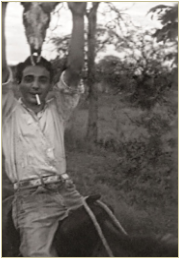
\includegraphics[width=0.6\linewidth]{19/no-pantanal.png}
\caption{Paulo no pantanal.}
\end{figure}

\begin{figure}
\centering
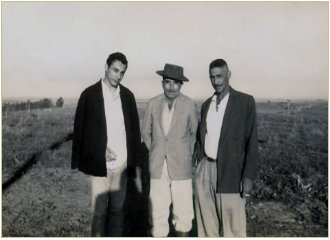
\includegraphics[width=0.85\linewidth]{19/comitiva.png}
\caption{Com os companheiros de comitiva.}
\end{figure}


\begin{figure}
\centering
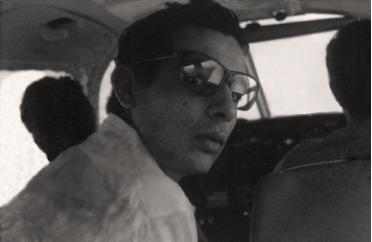
\includegraphics[width=0.85\linewidth]{19/voando+roberto.png}
\caption{Voando com Tio Roberto.}
\end{figure}

Não conheci outras pessoas cuja influência tenha sido decisiva na vida do Paulo.
Deve ter havido, mas não as conheci.
Mas, Yolanda, José Ignácio e Roberto conheci o suficiente para identificar de que maneira marcaram o seu jeito de ser.


Em comum, José Ignácio e Yolanda tinham a falta de limites e a dificuldade em orientar-se no mundo real.
Ela, por um ``panache'' que lhe era natural, não tinha medo de coisa alguma e não se curvava a nada.
A coragem nela era autêntica.
Mostrava ser, nos seus raros momentos de paz, uma grande entendedora da alma humana, lúcida e profunda, mas, nas fases de transtorno psíquico, seu humor e ironia, habitualmente tão sutis quanto divertidos, tornavam-se violentos e demolidores.
Então, não respeitava ninguém, fossem filhos, parentes, vizinhos, conhecidos, quem quer que se opusesse às suas vontades.


Era uma artista, fazia gravuras, delicadas pinturas e escrevia com graça e estilo.
Suas traduções do inglês, com as quais reforçava o orçamento após separar-se do marido, estão entre as melhores que já li.
Entretanto, tinha grande dificuldade em lidar com a realidade cotidiana e, principalmente, com as restrições que a vida de mãe de três filhos, separada de um marido psiquicamente desequilibrado e financeiramente instável, lhe impunham.
Tinha gostos sofisticados e, com alguma frequência torrava sua mesada quase instantaneamente com chás importados, bolos e queijos finos.
Além de montanhas de livros, claro.
Paulo conta que fazia coisas como receber a pensão do ex-marido, dinheiro que vez ou outra ela tinha de ir buscar na justiça, e contratar um táxi para levá-la ao litoral porque estava com vontade de velejar.
 

\begin{figure}
\centering
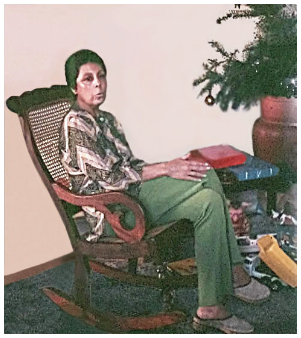
\includegraphics[width=0.8\linewidth]{19/d-yolanda.png}
\caption{D.Yolanda, por volta dos sessenta anos}
\end{figure}

Quando meus filhos eram pequenos e ela vinha visitar-nos, não conseguia conformar-se em ver-me enterrada naquela rotina de lecionar e cuidar dos meninos e da casa, entre fraldas e mamadeiras.
Dizia achar essa vida o cúmulo da mediocridade emburrecedora e andava atrás de mim, insistindo o tempo todo para que eu me sentasse para conversar sobre leituras e filmes.


Na sua própria casa, quando deixou José Ignácio e atravessou muitas fases de quase penúria, minha cunhada Marina conta, imitando-lhe o gesto refinado de sentar-se e acender um cigarro, que ela perguntava aos filhos, com cômica casualidade: - ``O que vocês acham de a gente abrir um bistrô?'' Sem levar em conta nem a falta de capital para tanto e nem o fato de que embora fizesse com certo domínio alguns pratos, cozinhava quando lhe dava na telha e sem muito critério.
Por exemplo, gostava de fazer um cozido português e o fazia bem.
Só que, quando isso acontecia, as crianças tinham que se preparar para comer o tal cozido a semana inteira, pois era só o que teriam até que ele acabasse.
Em José Inácio, a falta de limites e a valentia não me pareciam tão naturais e eu chego a acreditar que, embora lendárias, suas exibições em ambas as modalidades eram bastante seletivas -- só aconteciam quando ele se sentia seguro de que as circunstâncias, a surpresa ou a fraqueza do outro tornavam o revide improvável.
No fundo, constituíam-se apenas num \textit{mis-em-scène} destinado a obter para ele o reconhecimento de que carecia, orientado por um discutível senso de humor.
Porque a verdade é que José Ignácio era formalista ao extremo, reverenciava o poder e era grande apreciador das convenções sociais.
Gostava de vestir-se bem, era socialmente cavalheiresco no trato com as damas e revelava enorme apreço pelas tradições.
Era um cultor entusiasmado da genealogia paulista e suas origens familiares fincadas no bandeirantismo eram alardeadas \textit{ad nauseam}.
A desintegração da fortuna familiar que o atingiu na adolescência marcou-lhe fortemente a personalidade, com a adicional contribuição de uma mãe ``carola, ressentida e pouco iluminada'', conforme descrição da nora Yolanda.
Esta senhora, segundo minha sogra, descendente de tradicional família paulistana, enfrentou a perda do patrimônio na crise do café fazendo doces, quitandas e embutidos, com a ajuda das parentes, que mandava vender nas vizinhanças.
E José Ignácio, molecote ainda, era o escolhido para entregar as encomendas nas casas dos antigos colegas de brincadeiras e de escola.
Essa história de ter entregado, de porta em porta, as linguiças que a mãe fazia era recorrente nas suas reminiscências e parece ter contribuído para o sentimento de inadequação que dificultava sua relação com as pessoas.
Não que esse fosse um fato extraordinário numa época como aquela, de derrocada generalizada da aristocracia cafeeira.
O que, segundo minha sogra, marcou esse período a fogo na memória de José Ignácio foi a revolta sempre presente na fala, nos gestos e na expressão da mãe, D. Noêmia, inconformada por ver-se reduzida àquela condição.
É de se supor, também, que muita reza, muito conversa de culpa e castigo tenham sido ouvidas sob o teto daquela casa.
Porque Noêmia, sempre segundo Yolanda, responsabilizava o marido pela situação toda e atribuía a uma condenação divina as agruras que atormentavam a família.
Dois fatos testemunhados por mim, dão razão à minha sogra: o primeiro diz respeito à imensa quantidade de livros de oração antigos e muito manuseados pelas mulheres da família que eu vi na casa da irmã mais velha dele, Maria, logo após o falecimento dela e que eram representativos de uma rígida visão doutrinária, contemporânea da Contra Reforma ibérica; o outro, a menção constante que meu sogro fazia, nos seus últimos dias de vida, a punições e ao fogo do inferno e que surpreendia, numa pessoa informada como ele era, pelo que traduzia de uma visão física, concreta, da danação eterna instalada no seu inconsciente.
A relação culpa-castigo era muito firmemente plantada no ideário de José Ignácio.
Muito antes que as sucessivas isquemias fossem lhe restringindo a fala e os movimentos, a cada vez que morriam conhecidos ou parentes, ele costumava arrematar sua habitualmente cáustica análise da biografia do falecido, sentenciando: 
\textit{``-- Aqui se faz, aqui se paga!''}.

\begin{figure}
\centering
\includegraphics[width=0.8\linewidth]{19/yolanda+josé.png}
\caption{Yolanda e José Ignácio, recém-casados, passeando no Viaduto do Chá.}
\end{figure}

Arrisco-me a conjeturar que esta mentalidade seja a explicação plausível para o estoico silêncio com que suportou sua agonia final.
Ninguém conseguiu arrancar dele uma única queixa ou expressão de revolta.
Apenas ouvíamos o nome do filho, Paulo, chamado a toda hora como que para assegurar-se de tê-lo por perto, e curtos, e intensos gritos intermitentes que ele negava serem de dor.

\begin{figure}
\centering
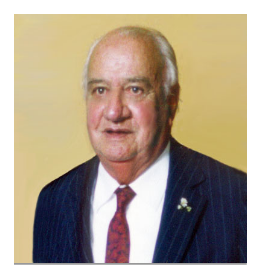
\includegraphics[width=0.8\linewidth]{19/josé.png}
\caption{José Ignácio, aos oitenta anos.}
\end{figure}

Ainda hoje, quarenta e um anos passados do dia em que conheci Paulo, posso dizer que ele esconde muitos enigmas que ninguém ainda desvendou.
Acredito que nem ele.
Porque Paulo parece não gostar de olhar para dentro de si mesmo e nem gosta de ser examinado de perto.
Sua permanente ansiedade trai medo e insegurança constantes cuja origem é fácil adivinhar, quando se conhece um pouco da sua história.
No entanto, disso mesmo provém sua grandeza.
Desconheço alguém que ao longo da vida tenha demonstrado tamanha coragem e persistência em enfrentar a própria fragilidade.
E, para mim, essa é a única medida que conta quando se avalia um ser humano.
Considerar a partir de onde e em que condições lançou-se na vida e verificar até onde conseguiu chegar.
Paulo, à meu ver, foi jogado no mundo sem a única defesa eficiente com a qual um indivíduo precisa contar -- a de ser reconhecido na infância, que permite a alguém saber quem de fato é.
Levando, além disso, na parca bagagem, instruções e mapas pouco confiáveis.
Aprendeu com a vida, literalmente.
Quase sozinho, por ensaio e erro.
E sobreviveu.
Foi longe, abriu caminhos, ousou, caiu e levantou.
Várias vezes.
Merece respeito.
Conseguiu ser o pai que ele nunca teve e, com sua experiência, pôde dar aos filhos o impulso necessário para que avancem até muito longe e com a serenidade e a confiança que ele próprio nunca experimentou.


\begin{figure}[H]
\centering
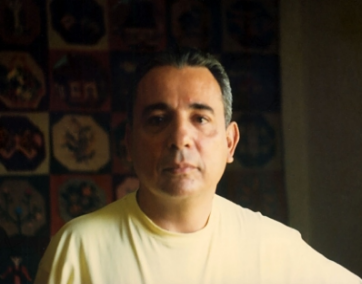
\includegraphics[width=0.9\linewidth]{19/paulo.png}
\caption{Paulo aos cinquenta anos.}
\end{figure}